\chapter{Phase-conjugate optical coherence tomography}

The past two decades have witnessed a number of experiments focused on the use of quantum-entangled states of light to achieve enhanced measurement capability in metrology. For example, quantum optical coherence tomography (Q-OCT) proposed by Abouraddy et al. \cite{abouraddy-qoct} and later demonstrated by Nasr et al. \cite{nasr-qoct}, utilized maximally entangled photon states and Hong-Ou-Mandel interferometry \cite{hong-interference} to achieve a 2$\times$ axial resolution improvement and dispersion cancellation over standard conventional OCT.

Such effects, including the enhanced resolution afforded by the width of the Hong-Ou-Mandel interference, and dispersion cancellation \cite{steinberg-dispersion,franson-dispersion}, were initially thought to be distinctly non-classical. However, much of the early research overlooked the possibility of classical light sources that possess no entanglement but are nevertheless maximally correlated in the classical, stochastic sense. Recent advances in nonlinear optical crystals and a better understanding of parametric downconversion have permitted us to generate a variety of these interesting classical light fields that bear properties previously associated exclusively with quantum optics. Of particular note is the ability to generate classical states with classically-maximal phase-sensitive correlations.

In particular, in the case of Q-OCT, Erkmen and Shapiro \cite{erkmen-pcoct} have shown that both the 2$\times$ axial resolution improvement and dispersion cancellation are not exclusively quantum effects, but merely a result of the phase-sensitive cross-correlation between the signal and idler of the biphoton state. This leads to the question of whether the same advantages can be obtained from an experiment with classical phase-sensitive light sources, which are uncommon but can be experimentally constructed. Erkmen and Shapiro proposed such a technique \cite{erkmen-pcoct}, called phase-conjugate optical coherence tomography (PC-OCT) which uses an unconventional arrangement using only classical light sources and classical photodetectors to achieve both of these advantages previously associated with Q-OCT.

In this chapter we explore classical, quantum, and phase-conjugate OCT configurations, build a parametric downconversion-based source to generate classical phase-sensitive light, and use it to implement PC-OCT.

\section{Optical coherence tomography configurations}

Optical coherence tomography (OCT) is a three-dimensional imaging technique that employs interference measurements to derive axial resolution. We explore three main techniques by which this is accomplished: conventional OCT (C-OCT), quantum OCT (Q-OCT), and phase-conjugate OCT (PC-OCT). In our analysis we disregard transverse scanning, and focus solely on axial (depth) resolution which is the differentiating aspect of the three methods.

\subsection{Conventional OCT}

The basic principle of C-OCT is shown in Figure \ref{figure:pcoct-schematic-coct}. C-OCT uses classical signal and reference light beams that have phase-insensitive cross-correlations, as might be generated using any classical high-flux source with a short coherence length (such as an LED or pulsed laser source) and a 50/50 beamsplitter. The signal beam interrogates the sample and the reflected light is recombined with the reference beam using a simple Michelson interferometer to measure the second-order correlations between the two beams. As the path length of either beam is scanned, the interference envelope reflects the axial profile of the target.

\begin{figure}[t]
\begin{center}
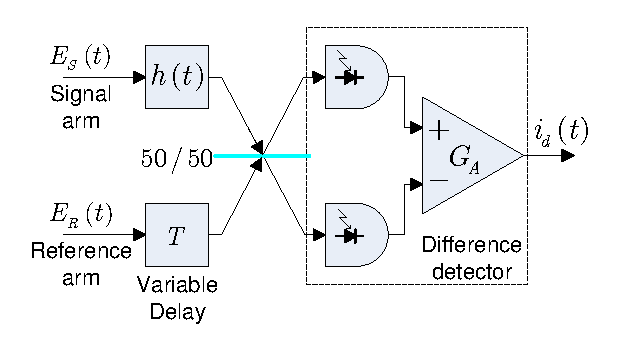
\includegraphics[width=13cm]{figure-pcoct-schematic-coct.pdf}
\caption{Schematic of conventional optical coherence tomography (C-OCT).}
\label{figure:pcoct-schematic-coct}
\end{center}
\end{figure}

Erkmen describes in \cite{erkmen-thesis} the analytic computation of the interference signature of C-OCT, which we briefly summarize here. We assume classical zero-mean, stationary, jointly Gaussian signal and reference fields with complex envelopes $E_S(t)$ and $E_R(t)$ with powers $\bar{h}\omega_0|E_K(t)|^2$ for $K = S, R$, respectively. In the case of C-OCT there are no phase-sensitive cross-correlations, and these fields are completely characterized by their phase-insensitive auto- and cross-correlations:

\begin{equation}
\langle E_J^*(t+\tau) E_K(t) \rangle = F^{-1}[S(\Omega)]
\end{equation}

for $J, K = S, R$ where

\begin{equation}
F^{-1}[S(\Omega)] = \int_{-\infty}^{\infty} \frac{d\Omega}{2\pi} S(\Omega) e^{i \Omega r}
\end{equation}

is the inverse Fourier transform of $S(\Omega)$ and $S(\Omega) = S(-\Omega)$ is the common spectrum of the signal and reference beams at $\pm\Omega$ from the center frequency $\omega_0$. We assume a target with an axial profile $h(t)$ and baseband impulse response $H(\Omega) = F[h(t)]$. In the case of a weakly reflecting mirror located at time delay $T_0$ and complex reflectivity $r$ with $|r| \ll 1$, this baseband impulse response is defined by:

\begin{equation}
H(\Omega) = re^{i(\omega_0 + \Omega)T_0}\,\,.
\end{equation}

After the signal field $E_S(t)$ interacts with the sample, the resulting field is described by the convolution of $E_S(t)$ with $h(t)$. An interferometric measurement is then made with the reference beam $E_R(t)$ delayed by time $T$. As shown by Erkmen and Shapiro \cite{erkmen-pcoct}, the resulting interferometric envelope is given by

\begin{equation}
\langle i_d(t) \rangle = 2q\eta G_A Re\left( \int_{-\infty}^{\infty} \frac{d\Omega}{2\pi} H^*(-\Omega) S(\Omega) e^{-i(\Omega-\omega_0)T}   \right)\,\,.
\end{equation}

Note that this envelope is linear in $H(\Omega)$. If we insert the response of the weakly reflecting mirror, we obtain an envelope proportional to $e^{-\Omega_S^2 (T_0 - T)^2 / 2}$. For a source with bandwidth $\Omega_S$, this gives us an axial resolution of $4/\Omega_S$, where we define resolution as the full-width between the $e^{-2}$ attenuation points of the visibility envelope.

Note also that C-OCT is vulnerable to dispersion in the sample, which will manifest itself inside $H(\Omega)$. Due to the linear dependence on $H(\Omega)$, there will be no dispersion-cancelling properties in C-OCT.

\subsection{Quantum OCT}

In Q-OCT, first proposed by Abouraddy et al. \cite{abouraddy-qoct}, the signal and reference beams are replaced by an entangled biphoton source and the Michelson interferometer is replaced by a Hong-Ou-Mandel (HOM) interferometric measurement \cite{hong-measurement}, as shown in Figure \ref{figure:pcoct-schematic-qoct}. In order to analyze Q-OCT we must use the quantum description of the fields. Suppose we have signal and reference beams with photon-unit field operators $\hat{E_S}(t)$ and $\hat{E_R}(t)$, respectively, with commutators

\begin{figure}[t]
\begin{center}
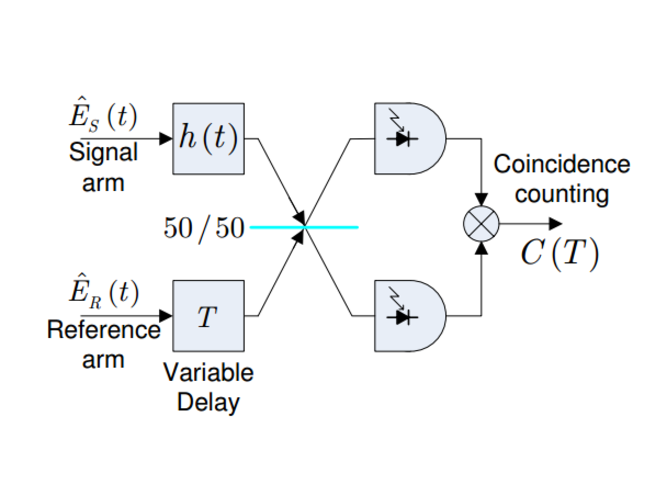
\includegraphics[width=13cm]{figure-pcoct-schematic-qoct.pdf}
\caption{Schematic of quantum optical coherence tomography (Q-OCT).}
\label{figure:pcoct-schematic-qoct}
\end{center}
\end{figure}

\begin{equation}
[ \hat{E_J}(t), \hat{E_K}^+(u) ] = \delta_{JK} \delta(t-u)
\end{equation}
for $J, K = S, R$. We further assume that the fields have the maximum phase-sensitive cross-correlation permitted by quantum mechanics:
\begin{equation}
\langle \hat{E}_S(t+\tau) \hat{E}_R(t) \rangle = F^{-1} [\sqrt{S(\Omega)(S(\Omega) +1)}]\,\,.
\end{equation}
Under these conditions, and in the biphoton limit (low photon flux) where HOM is usually performed, $S(\Omega)$ and the photon coincidence counting signature is shown by Erkmen and Shapiro \cite{erkmen-pcoct} to be:
\begin{equation}
\langle C(T) \rangle = \frac{q^2\eta^2}{2} \left[ \int_{-\infty}^{\infty} \frac{d\Omega}{2\pi} |H(\Omega)|^2 S(\Omega) - Re\left( \int_{-\infty}^{\infty} \frac{d\Omega}{2\pi} H^*(-\Omega)H(\Omega)S(\Omega)e^{-i2\Omega T} \right) \right]\,\,.
\label{equation:pcoct-qoct-envelope}
\end{equation}
Using the same partially-reflecting mirror, the dip in the coincidence counts is proportional to  $e^{-2\Omega_S^2 (T_0 - T)^2}$ Note that by the same resolution definition, we obtain an axial resolution of $2/\Omega_S$ which is twice the resolution as C-OCT for the same source bandwidth $\Omega_S$. Moreover, note that unlike C-OCT, the HOM dip term of Eq. \ref{equation:pcoct-qoct-envelope} is nonlinear in $H(\Omega)$ and involves a phase conjugation which will result in the cancellation of all even-order dispersion in the sample.

\subsection{Phase-conjugate OCT}

Although advantages of Q-OCT were earlier attributed to quantum effects, Erkmen and Shapiro showed that they are merely results of the phase-sensitive coherence between the signal and idler and achievable using PC-OCT \cite{erkmen-pcoct}, whose conceptual block diagram is shown in Figure \ref{figure:pcoct-schematic-pcoct}. In this configuration, the signal and idler are classical sources with phase-sensitive cross-correlations. The sample is interrogated twice at the same point with phase conjugation between the two passes.

\begin{figure}[t]
\begin{center}
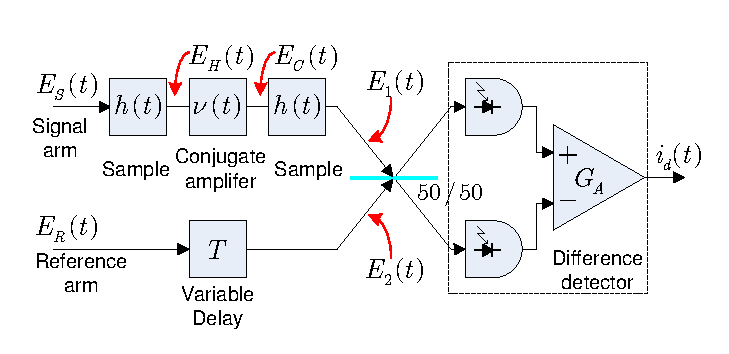
\includegraphics[width=13cm]{figure-pcoct-schematic-pcoct.pdf}
\caption{Schematic of phase-conjugate optical coherence tomography (PC-OCT).}
\label{figure:pcoct-schematic-pcoct}
\end{center}
\end{figure}

In PC-OCT, we assume classical signal and idler fields $E_S(t)$ and $E_R(t)$ with maximal phase-sensitive correlations as permitted by classical physics. The signal beam $E_S(t)$ is focused on a target with axial profile $h(t) = F^{-1}[H(\Omega)]$. The resulting field is
\begin{equation}
E_H(t) = E_S(t) * h(t)
\end{equation}
where $*$ denotes convolution. We then pass $E_H(t)$ into a conjugate amplifier with impulse response $v(t)$, resulting in the field:
\begin{equation}
E_C(t) = \left[ E_H^*(t) + w(t) \right] * v(t)
\end{equation}
where $w(t)$ is zero-mean white Gaussian quantum noise injected by the conjugation process, satisfying $TODO$, and $v(t)$ is the impulse response of the conjugator. After conjugation, the light is focused onto the same sample a second time, resulting in the field
\begin{equation}
E_1(t) = \left[ E_C(t) * h(t) \right] * e^{-i\omega_0 t}\,\,.
\end{equation}
We then recombine $E_1(t)$ with the reference beam, delayed by $T$, in a Michelson interferometer, yielding an interference signature of
\begin{equation}
\langle i_d(t) \rangle = 2q\eta G_A Re \left( \int_{-\infty}^{\infty} \frac{d\Omega}{2\pi} H^*(-\Omega)H(\Omega)V^*(-\Omega)S(\Omega) e^{-i(\Omega-\omega_0)T} \right)\,\,.
\end{equation}
This interference signature bears much resemblance to the second term of the interference signature of Q-OCT; both PC-OCT and Q-OCT have $H^*(\Omega)H(-\Omega)$ dependence. Indeed, if we use the same $H(\Omega)$ of the low-reflectivity mirror, we obtain a visibility function proportional to $e^{-2\Omega_S^2(T_0 - T/2)^2}$ and axial resolution of $2/\Omega_S$, which is identical to the resolution afforded by Q-OCT. In addition, the $H^*(\Omega)H(-\Omega)$ dependence of PC-OCT will result in even-order dispersion cancellation. Thus, PC-OCT realizes both of these advantages of Q-OCT with an entirely classical experiment.

It is also worth noting that PC-OCT can be (or may even preferably be) operated in a high-flux regime while Q-OCT cannot, since Q-OCT requires interference between individual photons and coincidence counting in order to perform the measurement. PC-OCT relies solely on classical interferometry, and thus is operable under a much wider range of conditions, including broad daylight, and data acquisition can be performed rapidly with classical detectors without large dwell times at each axial position.

\section{Generating phase-sensitive light with parametric downconversion}

Spontaneous parametric downconversion (SPDC) in nonlinear crystals was first observed in the 1960's and its properties extensively studied since then \cite{louisell-spdc,harris-spdc,magde-spdc,akhmanov-spdc,byer-spdc,burnham-spdc,tapster-spdc}. Recently, SPDC has been of particular interest to quantum optics experiments, particularly to generate heralded single photons \cite{fasel-spdc,pittman-spdc} and entangled photons \cite{kurtsiefer-spdc,wong-spdc}. However, while SPDC is useful in the weakly-pumped regime for quantum optics, few works have exploited the strongly-pumped regime for its strong classical phase-sensitive coherence between the signal and idler beams, which we make use of to implement PC-OCT.

\subsection{Single-mode parametric fluorescence}

We would like to couple our SPDC outputs into a single-mode fiber to ensure maximal phase-sensitive cross-correlations between the signal and idler outputs, as well as for the experimental convenience afforded by fiber optics. As SPDC output is typically highly multi-modal, a number of studies \cite{ljunggren-focus,kurtsiefer-spdc,bovino-focus,bennink-focus,fedrizzi-focus,boyd-focus} have explored the idea of manipulating the focusing of the pump beam to concentrate the majority of SPDC output into a single spatial mode. Based on analysis from these earlier studies \cite{legouet-interferometry}, we set our pump focusing parameter to $\xi_p = L/(k_p w_p^2) = \pi/2$ where $w_p$ is the pump waist size and $k_p$ is the wavenumber of the pump beam. However, a later and more comprehensive study by Bennink \cite{bennink-optimal} which was later supported by results by Dixon et al. \cite{dixon-heralding} shows that under the approximation that the focusing parameters of the signal, idler, and pump are similar ($\xi_s \approx \xi_i \approx \xi_p \approx \xi$), the joint spectral density of the signal and idler $|\psi(\omega_s, \omega_i)|^2$ is proportional to:
\begin{equation}
|\psi(\omega_s, \omega_i|^2 \propto F(\xi,\Phi) = \int_{-1}^1 \frac{\sqrt{\xi} \exp(i\Phi l/2)}{1-i\xi l} dl
\end{equation}
where $\Phi$ is the phase mismatch of the crystal. This is maximized for $\xi \approx 2.84$ and $\Phi \approx -1.04\pi$, yielding $F \approx 2.06$. In our suboptimal focusing case of $\xi = \pi/2$, $F(\xi = \pi/2, \Phi)$ is maximized for $\Phi \approx -0.75\pi$, yielding $F \approx 1.96$, implying that we our joint spectral density is $\sim$5\% less than optimal.

\begin{figure}[t]
\begin{center}
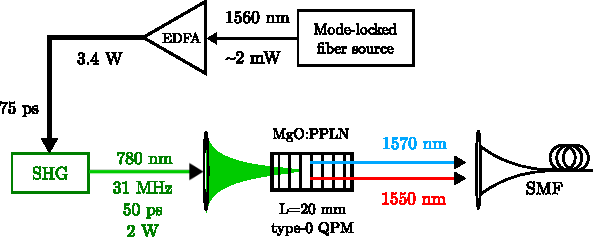
\includegraphics[width=13cm]{figure-pcoct-setup-spdc.pdf}
\caption{Schematic of setup for parametric fluorescence generation and collection in single-mode fiber. We use type 0 phase matching (signal, idler, pump are polarized on the same axis) in a MgO:PPLN crystal.}
\label{figure:pcoct-setup-spdc}
\end{center}
\end{figure}

Figure \ref{figure:pcoct-setup-spdc} shows a schematic of the SPDC generation setup. A home-built passively mode-locked pulsed Er-doped fiber laser employing polarization-maintaining fiber \cite{venkatraman-thesis} was used as a seed source. The center wavelength of 1560 nm was set by a Bragg grating within the laser cavity. The laser generated 75-ps pulses at a repetition rate of $\sim$31.1 MHz and average output power of $\sim$1.9 mW, with an output spectrum shown in Figure \ref{figure:pcoct-seedspectrum}. This seed laser output was fed into an IPG Photonics Er-doped fiber amplifier (EDFA) with a maximum output of ~6 W. In practice, we set the amplifier output power to a lower setting (typically 3-4 W) to avoid the effects of self-phase modulation (SPM), which at high power levels distorts the pulse shape and destroys the transform-limited properties of the pulse. In order to further reduce the effect of SPM, we had the EDFA serviced by IPG Photonics to reduce the internal fiber length to a bare minimum. The spectrum of the output at maximum power setting, before and after modification, is shown in Figure \ref{figure:pcoct-edfabeforeafter}. The EDFA output power showed linear behavior as a function of drive current, after a minimum threshold of $\sim$400 mA, as shown in Figure \ref{figure:pcoct-edfapower}.

\begin{figure}[h]
\begin{center}
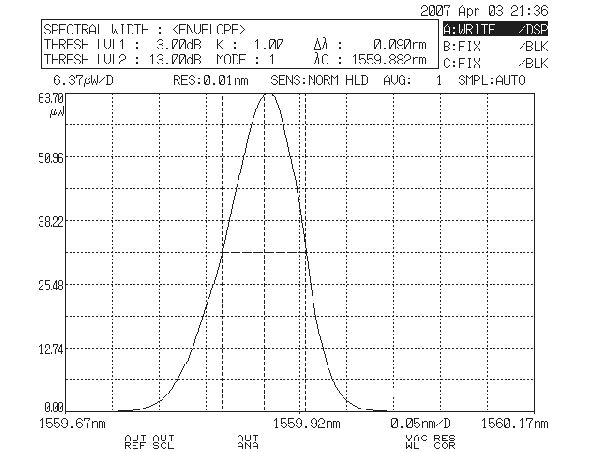
\includegraphics[width=13cm]{figure-pcoct-seedspectrum.pdf}
\caption{Spectrum of a home-built passively mode-locked fiber laser \cite{venkatraman-thesis} used as a seed source.}
\label{figure:pcoct-seedspectrum}
\end{center}
\end{figure}


\begin{figure}[h]
\begin{center}
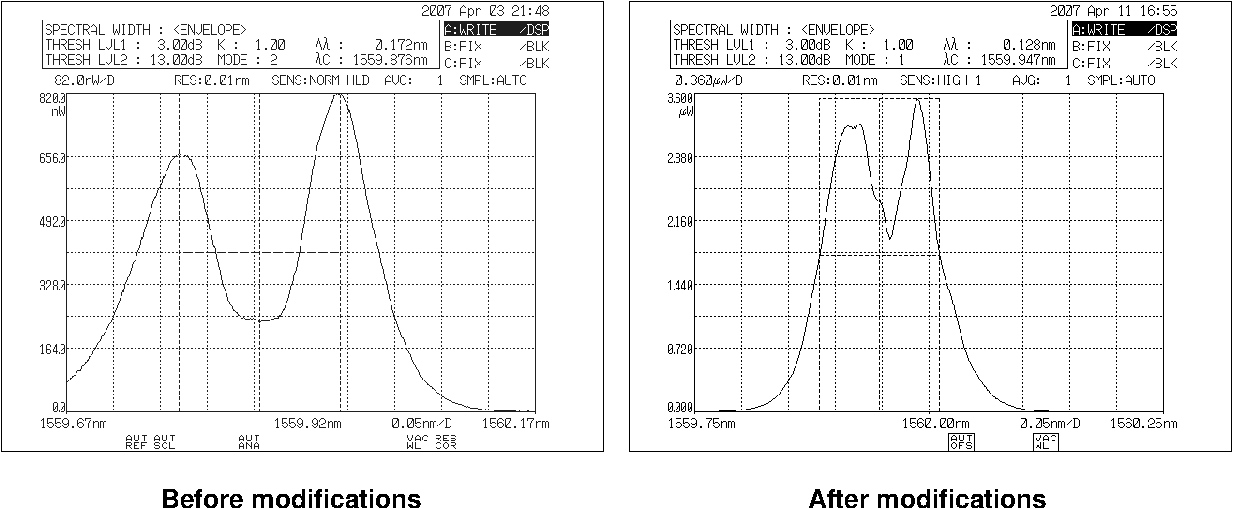
\includegraphics[width=16cm]{figure-pcoct-edfabeforeafter.pdf}
\caption{EDFA output spectrum at maximum output power setting, before and after modifications by IPG Photonics to remove excess internal fiber. The broadening of the spectrum and double peak is caused by self-phase modulation inside the fiber at high power levels.}
\label{figure:pcoct-edfabeforeafter}
\end{center}
\end{figure}

\begin{figure}[h]
\begin{center}
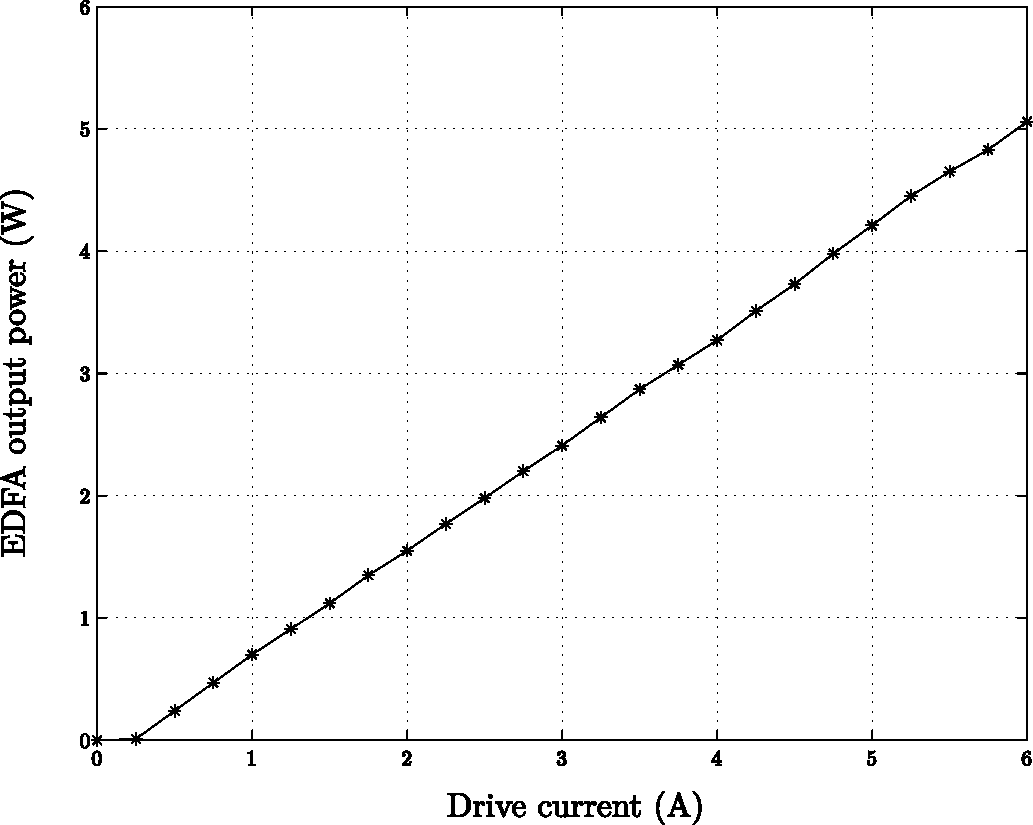
\includegraphics[width=10cm]{figure-pcoct-edfapower.pdf}
\caption{EDFA output power (1560 nm) as a function of drive current, showing linear behavior with a threshold of $\sim$400 mA.}
\label{figure:pcoct-edfapower}
\end{center}
\end{figure}

\begin{figure}[h]
\begin{center}
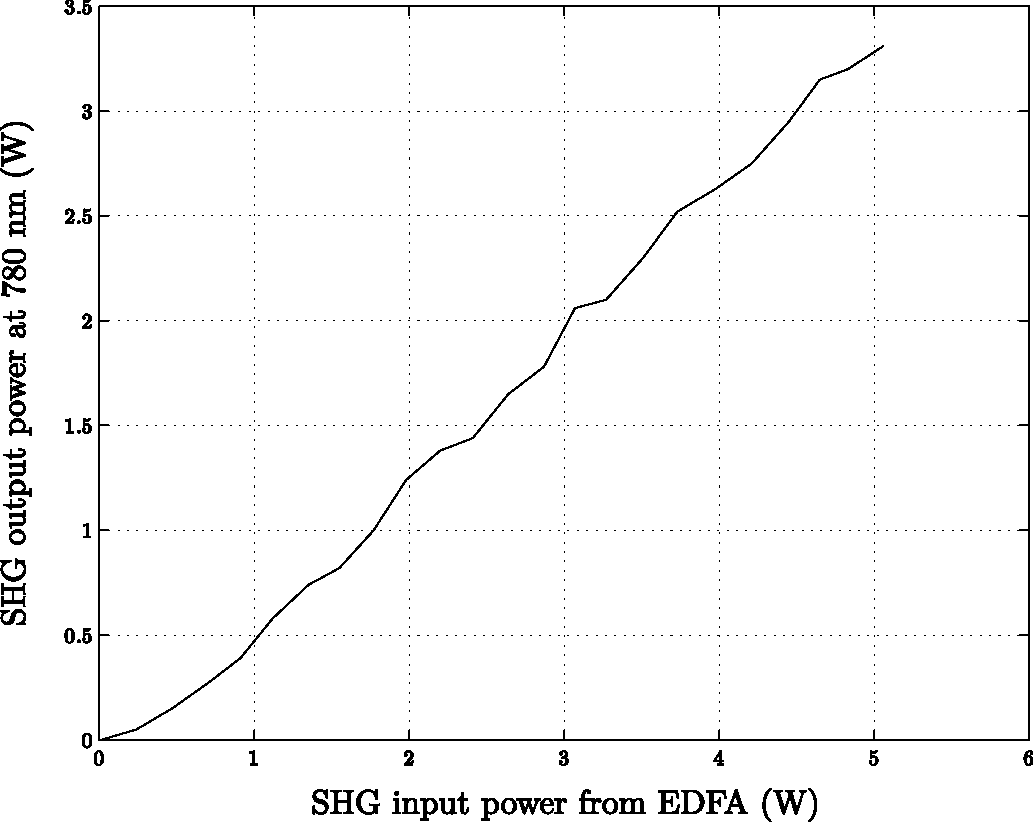
\includegraphics[width=10cm]{figure-pcoct-shg.pdf}
\caption{SHG output power (780 nm) as a function of input power (1560 nm), showing quadratic dependence at low power levels and linear dependence at high power levels.}
\label{figure:pcoct-shg}
\end{center}
\end{figure}

We then frequency-doubled the free-space output of the EDFA using a MgO:PPLN crystal with a grating period of 19.47 $\mu$, housed in a temperature-controlled oven set at ~86.5$^\circ$C, which was phase-matched to produce ~50-ps pulses at 780 nm by second harmonic generation (SHG). By focusing the input into the crystal to a waist of 40 $\mu$m and careful optimization of the temperature we were able to convert 3.4 W of 1560 nm input into 2 W of output at 780 nm, indicating a conversion efficiency of 59\%. The SHG output power is quadratic in the input power in the low efficiency regime, but linear in the high efficiency regime, as shown in Figure \ref{figure:pcoct-shg}. Multiple dichroic mirrors were used to filter out the remaining 1560 nm light. Since we intend to use the 780 nm light to pump an SPDC source at 1560 nm with a second nonlinear crystal, it is important that the strong leftover 1560 nm light from the EDFA is almost completely filtered out with a sufficient number of dichroic mirrors after the SHG stage; we placed enough diochroic mirrors to attenuate the residual 1560 nm power to under 1 nW.

We then optimized the pump focusing for the SPDC using our earlier theoretical estimates as a starting point by focusing the pump to a waist of 35 $\mu$m, which gives $\xi_p = \xi_t \sim 1$. With this focusing fixed, we optimize the coupling of the SPDC output into a single mode SMF-28 fiber, measuring the power at the other end of the fiber using a fiber-coupled InGaAs detector with 10-fW sensitivity. In order to measure the coupling efficiency, we also obtained the total SPDC output power by using a multi-mode fiber in its place. Using this initial setting, we obtained a ratio of $\eta_T = 50$\%. However, to account for the coupling losses and deduce the actual single-mode content of the SPDC output, we connected a single-mode 1550 nm fiber laser source to both our single- and multi-mode fiber inputs and obtained an efficiency of $\eta_{f} = 82 \pm 2$\%. Our SPDC single-mode content can then be deduced to be $\eta_{SM} = \eta_{T}/\eta_{f} = 61 \pm 1.5$\%.

We then varied the pump focusing and repeated the efficiency measurement at each setting. At a waist of $w_p = 25\,\mu$m we obtained $\eta_T = 57.5$\% and $\eta_{SM} = 70 \pm 2$\% which corresponds to $\xi_p = \xi_t = 1.7$. One crystal shattered under tight focusing conditions as the pump power was increased, after which we subsequently avoided attempting to focus the pump too tightly as a precaution. However, as described above, later work by Bennink \cite{bennink-optimal} indicates that tighter focusing may have yielder better results.

\subsection{SPDC under strong pumping}

SPDC is traditionally used in the low-flux regime to generate biphoton and entangled photon states. However, in this experiment we are interested not in the quantum properties of SPDC but merely the phase-sensitive cross-correlations between the signal and idler. Thus, it is useful to have strong pumping beyond this low-flux regime. While in the low-flux regime, the SPDC power output is linear in the pump power, as the pump power is increased sufficiently, the SPDC output enters a regime of exponential dependence, due to the parametric amplication of the parametric fluorescence itself before exiting the crystal. This parametric amplification incidentally also breaks any entanglement properties of the SPDC outputs, but  PC-OCT does not make use of quantum entanglement. In the amplified regime, the signal and reference beams continue to have classically-maximal phase-sensitive correlation which is sufficient for the experiment. Figure \ref{figure:pcoct-data-power} shows that for our setup, we enter this regime at pump powers greater than 0.5 W - 1 W. It is also worth noting that as we enter this regime, the SPDC output bandwidth increases linearly with pump power, shown in Figure \ref{figure:pcoct-data-spectrum}(b).


\begin{figure}[t]
\begin{center}
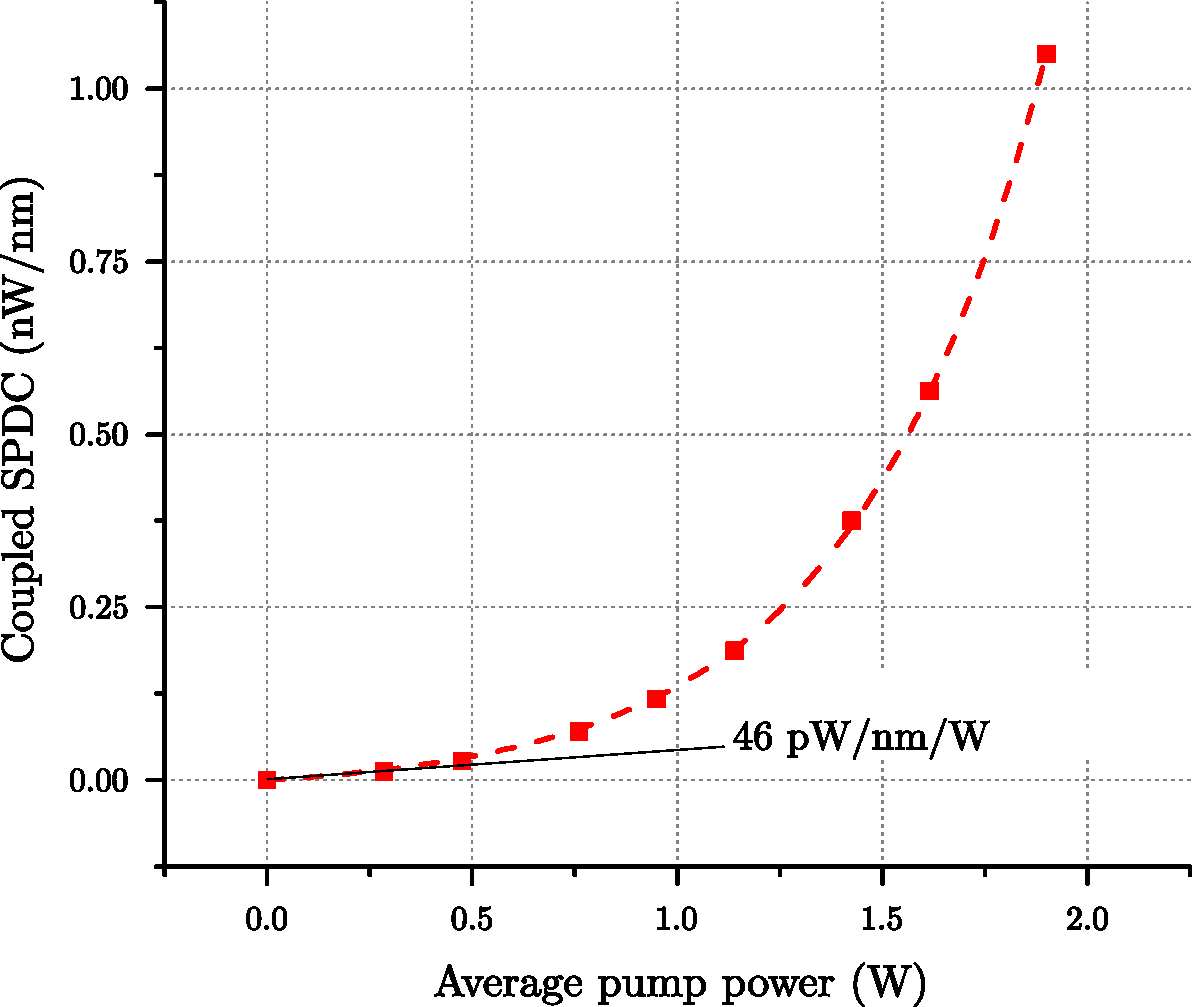
\includegraphics[width=10cm]{figure-pcoct-data-power.pdf}
\caption{SPDC output power as a function of pump power, showing the linear dependence in the low-flux regime and exponential dependence in the high-flux (amplified) regime.}
\label{figure:pcoct-data-power}
\end{center}
\end{figure}

\begin{figure}[t]
\begin{center}
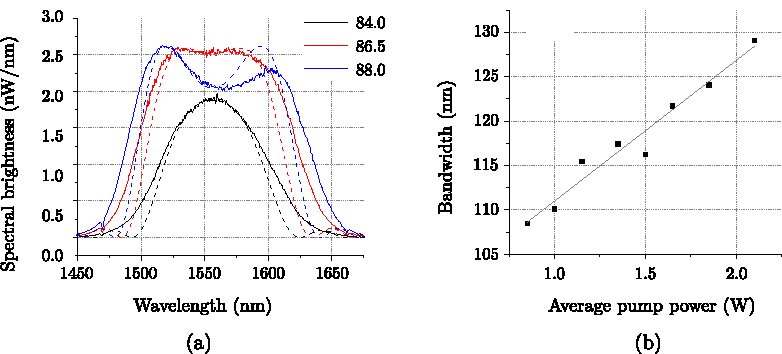
\includegraphics[width=\textwidth]{figure-pcoct-data-spectrum.pdf}
\caption{(a) Power spectral densities (solid) and theoretical models based on Sellemeier coefficients (dashed) for various crystal temperatures, with pump power fixed at 2 W. (b) Linear dependence of SPDC output bandwidth as a function of pump power, with temperature fixed at 86$^\circ$C.}
\label{figure:pcoct-data-spectrum}
\end{center}
\end{figure}


\section{Experimental setup}

\begin{figure}[t]
\begin{center}
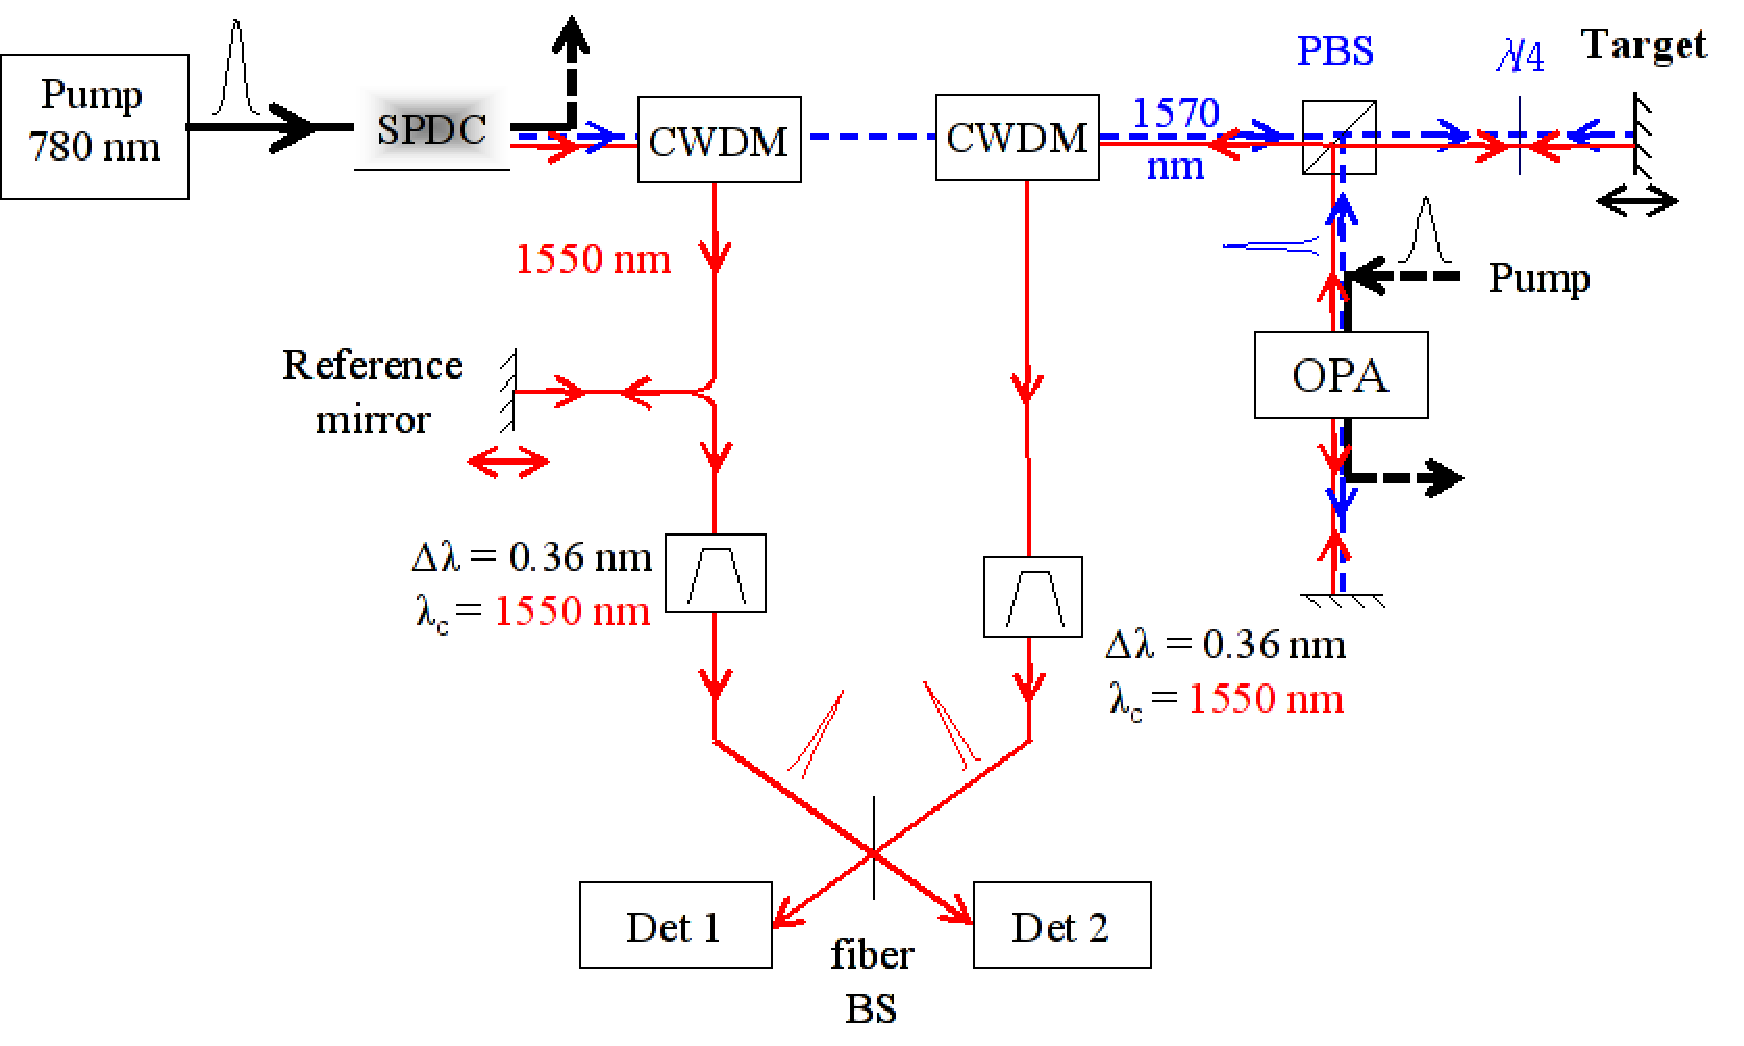
\includegraphics[width=16cm]{figure-pcoct-setup.pdf}
\caption{PC-OCT experimental setup. CWDM: course Wavelength division Multiplexer, OPA: optical parametric amplifier, PBS: polarizing beamsplitter.}
\label{figure:pcoct-setup}
\end{center}
\end{figure}

We now turn to using our SPDC-based phase-sensitive light source to demonstrate PC-OCT, with the setup shown in Figure \ref{figure:pcoct-setup}. We devised a method to interrogate the same sample twice with phase conjugation, a physical simulation of sample dispersion using a long fiber spool to demonstrate dispersion cancellation, a classical interferometric measurement, and an automated positioning and data collection system.

\subsection{SPDC source}

We coupled the SPDC light previously described into the input of a 4-channel JDS Uniphase course wavelength division multiplexer (CWDM) with center wavelengths at 1530 nm, 1550 nm, 1570 nm, and 1590 nm, with nearly flat-top passbands of 16 nm at each channel, as shown in Figure \ref{figure:pcoct-cwdm}. We used the 1550 nm channel as the reference and the 1570 nm channel as the signal.

\subsection{Double-pass configuration and phase conjugation}

\begin{figure}[h]
\begin{center}
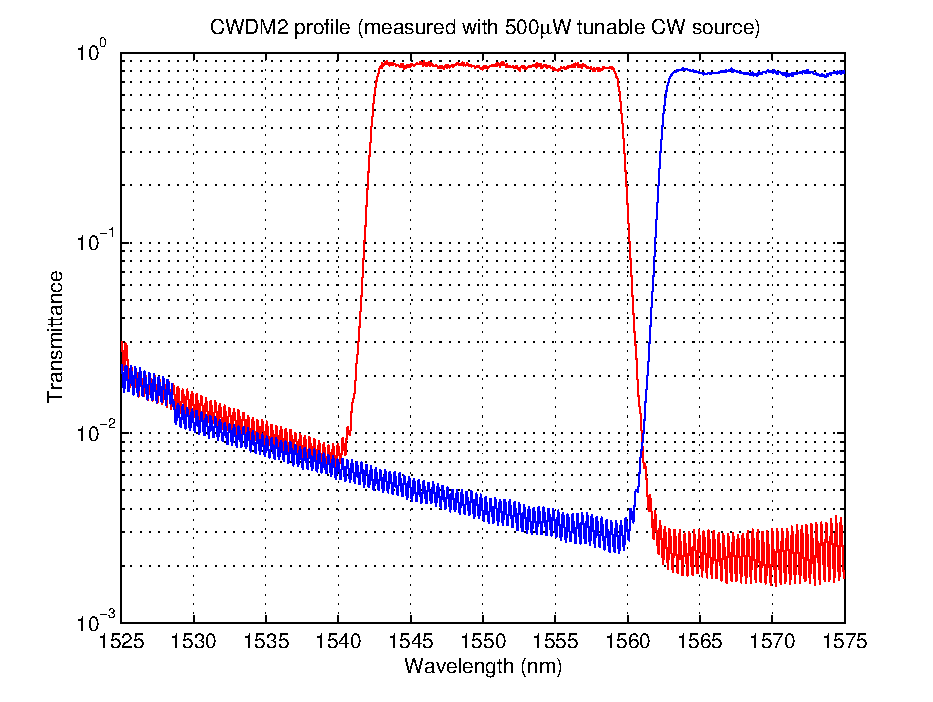
\includegraphics[width=12cm]{figure-pcoct-cwdm.pdf}
\caption{Transmittance of 1550 nm and 1570 nm channels of the CWDM, scanned using a InGaAs detector and tunable fiber-coupled laser with a maximum wavelength of 1575 nm, showing nearly flat-top transmission and sharp falloff, allowing the reference and signal to be efficiently separated.}
\label{figure:pcoct-cwdm}
\end{center}
\end{figure}

PC-OCT requires that the signal light passes through the same target twice before an interference measurement with the idler beam. We accomplished this double-pass configuration using a polarizing beamsplitter (PBS) and quarter-waveplate as shown in Figure \ref{figure:pcoct-setup}. We first sent the 1570-nm light from the first CWDM to a second CWDM that is configured in reverse (i.e., light was injected into the 1570 nm channel and exited at the common port). We then collimated the output and configured it to be horizontally polarized using polarization control paddles. The horizontally polarized light then passed through a polarizing beamsplitter (PBS) unreflected, followed by a quarter-waveplate, leaving it in a circular polarization before interacting with the target. The reflected light passed through the same waveplate on the return path, converting it to a vertical polarization, which upon returning to the PBS was reflected into an optical parametric amplifier (OPA) which performed the phase conjugation using a third MgO:PPLN crystal of the same poling period. Parametric amplification necessitates that the pulsed pump light and the pulsed return signal are matched in time, which we accomplished by re-using the residual 780 nm pulsed pump signal from the second (SPDC) crystal with a free-space variable delay. In this experiment, the 50-ps pump pulse limited the range of targets to a maximum axial displacement of $\sim$15 mm, beyond which parametric amplification would not occur, although it is in principle possible to translate the pump and target simultaneously to accomodate larger ranges.

The reflected, phase-conjugated light then followed the entire optical path in reverse and was re-coupled back into the second CWDM. Since the OPA was pumped at 780 nm, the wavelength of the phase-conjugated beam was 1550 nm and exited the second CWDM from its 1550 nm port, ready for interference measurement with the 1550 nm reference arm.

We additionally installed fiber-coupled filters on both reference and signal (after conjugation) arms. The filters have Lorentzian spectral profiles with widths of $\Delta\lambda = 0.36$ nm and tunable center wavelengths near 1550 nm, and transmission of $\sim$45\%, setting the measurement bandwidth narrow enough for signal and idler beams to be transform-limited.

\subsection{Dispersion simulation using long fiber spool}

At the pulse width of 50 ps we used in our experiment, typical free-space optics cannot easily provide sufficient dispersion to test the even-order dispersion-cancelling properties of PC-OCT; however, sample dispersion becomes a significant issue for OCT experiments involving thick samples and femtosecond lasers. For testing purposes, we simulate sample dispersion by inserting $\sim$50 meters of SMF-28 fiber (with a dispersion of 17 ps/nm/km) in the signal arm. In the reference arm, we do not wish to deliberately induce dispersion, but it is necessary to match the optical path length of the signal arm in order to perform an interferometric measurement. Since zero dispersion fiber is not widely available, we used Corning LEAF fiber, a widely-available nonzero dispersion-shifted fiber commonly used for telecommunications with a dispersion of $\sim$4 ps/nm/km at 1560 nm. Although this dispersion will not be cancelled by PC-OCT, it is much lower than the SMF-28 fiber used in the signal arm. The reference arm needed a total of 135 m of LEAF fiber to match the total optical length of SMF-28 in the signal arm. This length was measured by injecting pulses into both arms and performing time-of-flight measurement using high-speed InGaAs photodetectors.

We observed that the index of refraction of fiber was significantly affected by changes in the ambient temperature; the fluctuations in room temperature by $\pm 1^\circ$C were enough to cause several millimeters of difference in effective optical length after the $\sim$135 m of fiber length used in the experiment. We confirmed this by monitoring the changes in room temperature, as shown in Figure \ref{figure:pcoct-dpplot}, and alleviated the problem by placing the bulk of the fiber spool inside a thermally-insulating foam container, performing successive measurements within a short time frame, and monitoring the room temperature carefully to ensure consistent measurement conditions.

\begin{figure}[h]
\begin{center}
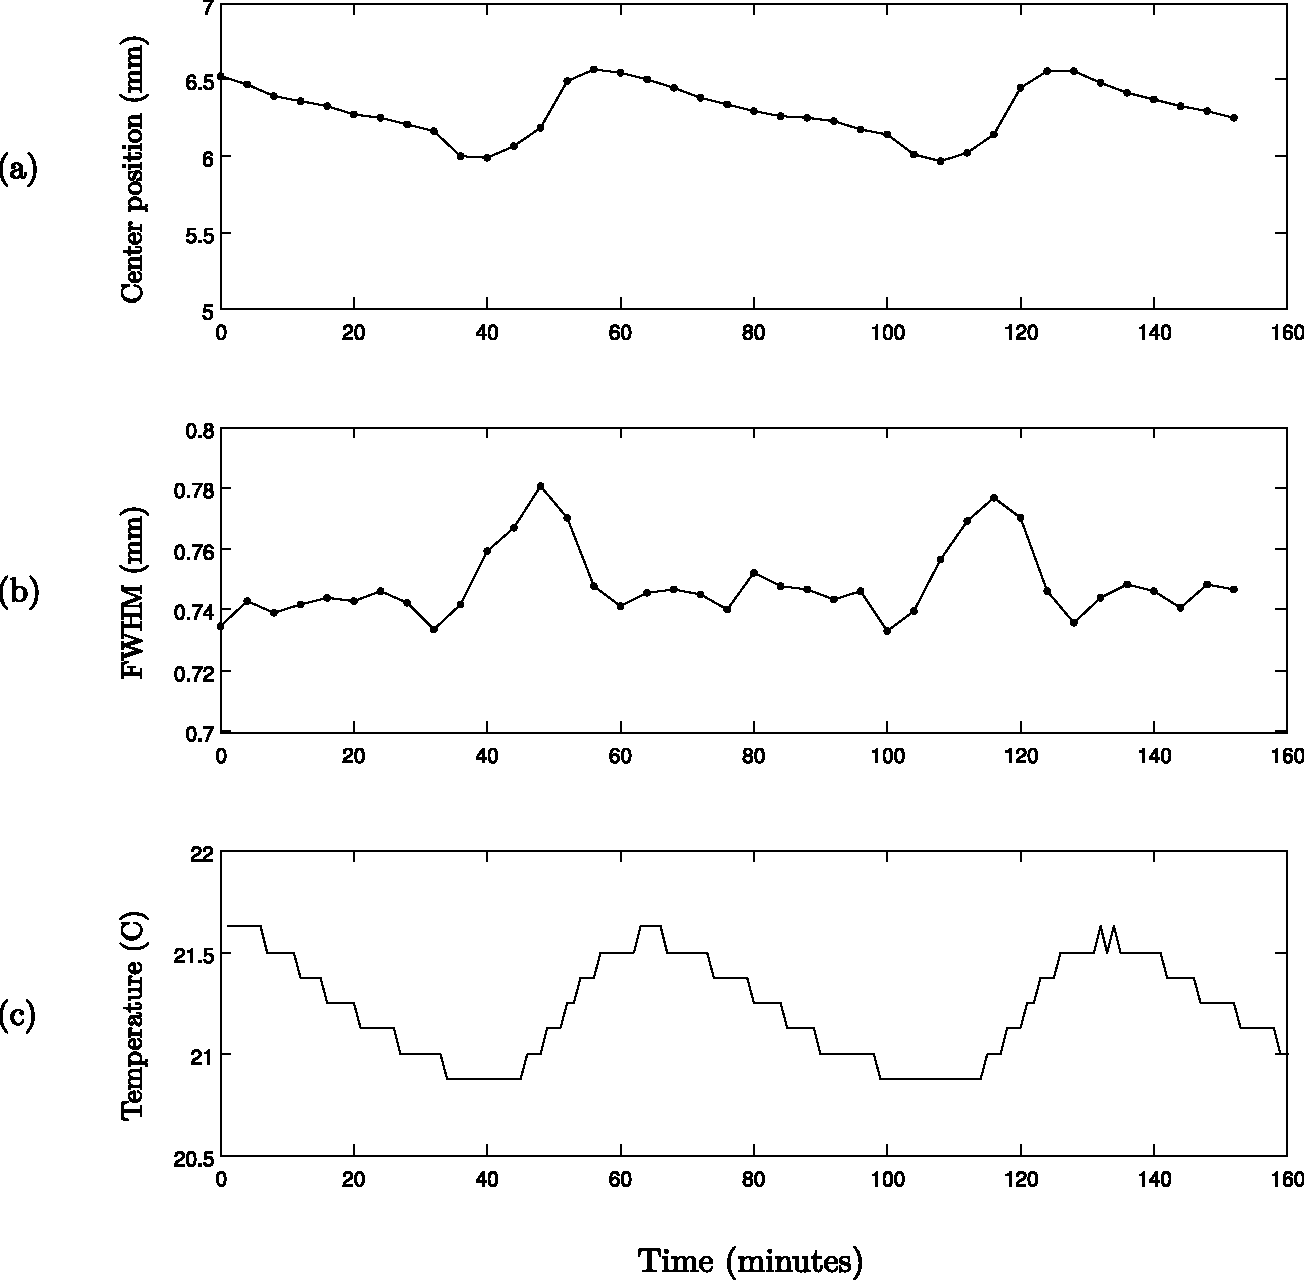
\includegraphics[width=13cm]{figure-pcoct-dpplot.pdf}
\caption{(a) Center position and (b) FWHM of the PC-OCT interferometric envelope, with (c) synchronized measurements of the ambient room temperature, showing the effect of temperature on the index of refraction of the long fibers in the experiment.}
\label{figure:pcoct-dpplot}
\end{center}
\end{figure}

\subsection{Interferometric measurement}

Interferometric measurement was performed by combining both signal and reference arms using a 50/50 fiber beam splitter. A fiber circulator and free-space delay facilitated the ability to fine-tune the optical path length difference of the two arms. A constantly swept piezoelectric transducer was added to the free-space delay in order to continuously scan the interferometer over a full wavelength at each position and measure the interference visibility. (TODO: show interference signal envelope sample)

\subsection{Data collection}

We connected both interferometer outputs to two channels of a high-sensitivity (0.1 pW) HP8163A InGaAs power meter, and linked to a computer via GPIB connection. A custom Visual Basic program was written to synchronously drive the PicoMotor stages and read values from both channels of the power meter. The PZT mirror was modulated at a frequency of 80 Hz, intentionally slower than the averaging time of the power meter, allowing the program to read the interference amplitude by logging a series of power values from the power meter with the stage stationed at any point. The interference amplitude was normalized to the sum of power outputs from both channels in order to compensate for laser power fluctuations.

\section{Results}

\begin{figure}[t]
\begin{center}
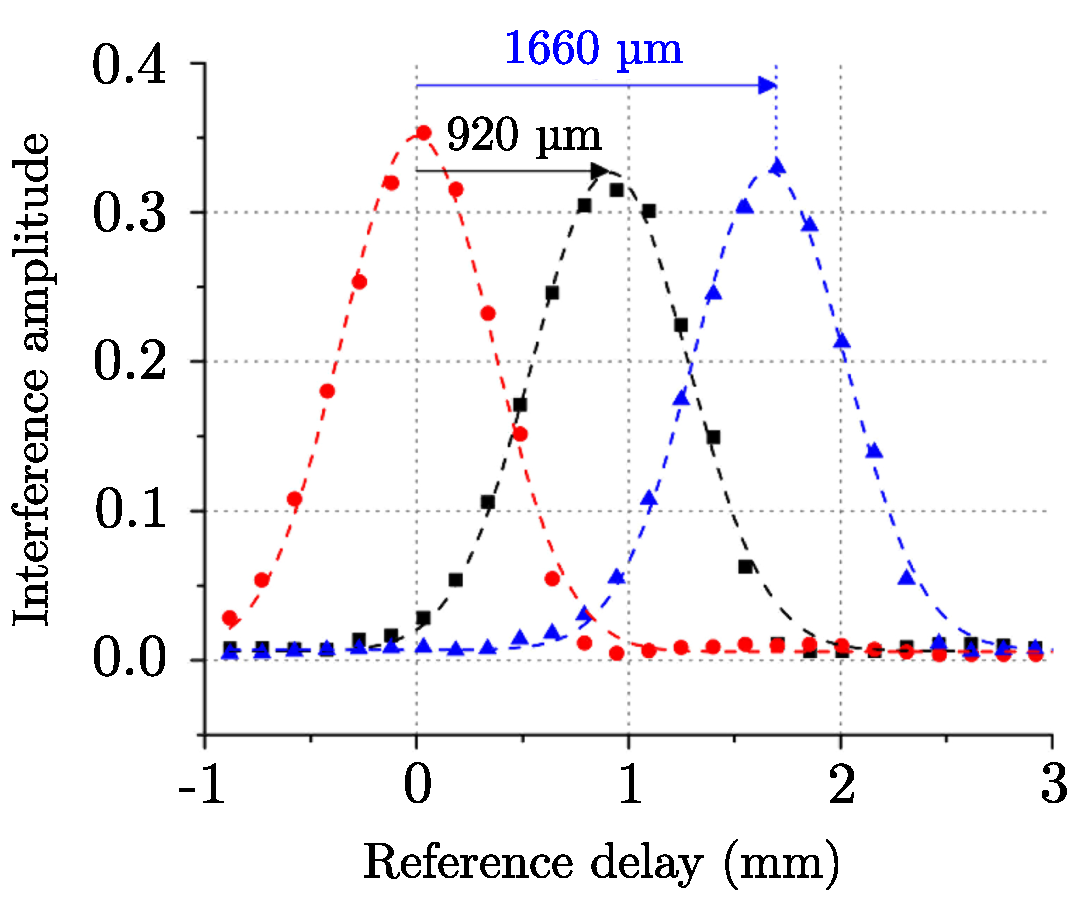
\includegraphics[width=12cm]{figure-pcoct-result.pdf}
\caption{Three PC-OCT scans with a high reflectivity mirror used as a target, translated by 450 $\mu$m between subsequent scans.}
\label{figure:pcoct-result}
\end{center}
\end{figure}

Using a high reflectivity mirror as a target, Figure \ref{figure:pcoct-result} shows the results of three successive scans of the target with a relative separation of $\Delta z$ = 450 $\mu$m. Given the double-pass configuration, one would expect the resulting peaks to have a relative separation of $\Delta z_R = 2\Delta z$ giving us a $2\times$ axial improvement. The observed shifts were 920 $\pm$ 20 $\mu$m and 1660 $\pm$ 20 $\mu$m, confirming this behavior; the discrepancy in the right peak from the expected $\sim 1800$ $\mu$m is likely attributable to room temperature fluctuation as described earlier. Note that this effect is particularly noticable because of the added long fibers for inducing dispersion.

In addition to the 2$\times$ axial resolution improvement, we expect to observe cancellation of even-order dispersion in the signal arm. The expected width of the interference envelope is given by the convolution of the signal and reference fields, accounting for dispersion:
\begin{equation}
L_{OCT}^2 = 4 L_0^2 + (c \Delta\lambda_F)^2 (D_S (z_{S1}-z_{S2}) + D_R z_R)
\end{equation}
where $z_{S1} = 77.1$ m is the length of fiber in the signal arm before conjugation, $z_{S2} = 71.2$ m is the length of fiber after conjugation (leaving a net 5.9 meters of fiber in which dispersion is not cancelled in the signal arm), $z_R = 135$ meters is the length of fiber in the reference arm, and $D_S$ and $D_R$ are the dispersion coefficients in the signal and reference arms, respectively. Since we intended to deliberately induce dispersion in the signal arm to demonstrate the dispersion-cancelling properties of PC-OCT, we used standard SMF-28 fiber which has $D_S = 17$ ps/nm/km. The length of fiber in the reference arm was chosen to match the signal arm for interometric measurement; we chose not to have a significant amount of dispersion in the reference arm, in order to demonstrate the dispersion-cancelling properties of the phase-conjugating signal arm. However, as zero-dispersion fiber was not available, we used LEAF fiber, a commonly-used nonzero dispersion shifted fiber (NZ-DSF) designed for telecommunications and with a dispersion of $D_R = 4.2$ ps/nm/km. Using these values, we obtain a predicted FWHM of $L_{OCT} = 893 \pm 30\,\mu$m which is in excellent agreement with the measured width of $890 \pm 30\,\mu$m. If dispersion had not been cancelled, we would flip the sign of $z_{S2}$:
\begin{equation}
L_{OCT}^2 = 4 L_0^2 + (c \Delta\lambda_F)^2 (D_S (z_{S1}+z_{S2}) + D_R z_R)\,\,.
\end{equation}
This yields $L_{OCT} = 3.02$ mm, over three times larger than our measured value, suggesting that dispersion cancellation was achieved almost perfectly in the signal arm.

We see that PC-OCT recovers both of the main advantages previously associated with Q-OCT using an entirely classical setup. In addition, Erkmen showed \cite{erkmen-thesis} that as long as the conjugator gain $|V|^2$ is large and reflected field strong, the signal-to-noise ratio (SNR) of PC-OCT is similar to that of C-OCT, which is expected since they employ a similar principle of operation. On the other hand, Q-OCT relies on SPDC to generate entangled photon states and thus necessitates operation at low flux and use of Geiger-mode avalanche photodetection to observe fourth-order Hong-Ou-Mandel interference, which significantly limits acquisition speed and operating conditions.

PC-OCT owes its resolution advantage to its double-pass configuration. However, an intimate relationship between this and Q-OCT can be seen in Abouraddy's interpretation of Q-OCT \cite{abouraddy-qoct} which accounts for the $H^*(\Omega)H(-\Omega)$ term as a product of an actual sample illumination and a virtual sample illumination, which in PC-OCT is manifested in two successive illuminations. PC-OCT's double-pass configuration providing an axial advantage over C-OCT also leads us to consider the possibility of C-OCT in a double-pass configuration, with phase-insensitive sources and no phase conjugation. In this case, although a resolution advantage would be obtained, even-order dispersion would be doubled instead of cancelled \cite{erkmen-pcoct}.

\section{Conclusions}

Recent developments in quantum optics have led to new methods in sensing that involve entangled biphotons and other nonclassical states of light to achieve advantages over their conventional counterparts. In particular, Q-OCT uses quantum interferometry to achieve a two-fold resolution improvement and even-order dispersion cancellation over C-OCT. Although these advantages have been proposed and demonstrated, we begin to question the true nature of the claimed advantages of these quantum techniques, whether those advantages are truly quantum in nature, and moreover, if there is an unconventional classical method to achieve the same results.

In particular, we demonstrate experimentally through PC-OCT that Q-OCT's advantages, although realizable using quantum interferometry, arise from the phase-sensitive cross-correlations in the signal and idler beams and are realizable using a novel classical technique. In addition, PC-OCT is operable at much higher light levels and acquisitions may be performed extremely rapidly, incorporating the best advantages of classical sensing.

In this work, we also address the experimental implementation issue of PC-OCT. Most classical light sources have only phase-insensitive cross-correlations and no phase-sensitive cross-correlations. Our setup requires strong and broadband phase-sensitive cross-correlations between signal and idler beams, which in principle can be produced by splitting a laser beam and imposing anti-correlated phase noises on both beams using modulators. However, in this work, we demonstrate an approach that employs nonlinear optics, which provide a bandwidth significantly higher than can be achieved using modulators. We consider the SPDC sources used to generate biphoton states with phase-sensitive cross-correlations for quantum optics experiments, but operated in a strong-pump, high-flux regime in which photons are amplified before exiting the crystal. Although this destroys their entanglement properties, the phase-sensitive cross-correlations are preserved perfectly which is sufficient to implement PC-OCT, which makes no use of quantum interference. We implemented such a source and carried out a PC-OCT experiment, demonstrating the realizability of strong, phase-sensitive classical light sources which, while unconventional, are not beyond the limits of classical physics, and may be useful for a variety of other sensing applications.


